\chapter*{Pitch perception - JND}

\section*{Introduction}
The purpose of this study is to evaluate the just noticeable difference (JND) of pitch.
Webers law:

\begin{equation}
\Delta I = k \cdot I
\end{equation}

\section*{Methods}
%
\begin{itemize}
  \item Psychometric method
  \item Method of Constant Stimuli
  \item Data collection method: Two-Alternative Forced Choice (2-AFC) (avoids criterium problems)
\end{itemize}


\subsection*{Stimuli}
%
\begin{itemize}
\item Reference stimulus intensity: 800 Hz (pure tones)
\item Expected JND: ca. 1.2 Hz (Wier, Jesteadt \& Green, 1977)
\item Logarithmic distribution on chosen frequencies from a 800 Hz reference.
\item Difference from 800 Hz: 0.3 Hz, 0.6 Hz, 1.2 Hz, 2.4 Hz, 4.8 Hz, 9.6 Hz. (before pilot test)
\item Order of stimuli representation: Randomize presentation order for comparisons over all frequencies and repetitions.
\item Repetitions: 12 at each frequency 
\end{itemize}


\subsection*{Experimental setup}
Equipment: Bang \& Olufsen H6 headphones, Lenovo ThinkPad (Volume 10\%)

\begin{figure}[H]
\centering
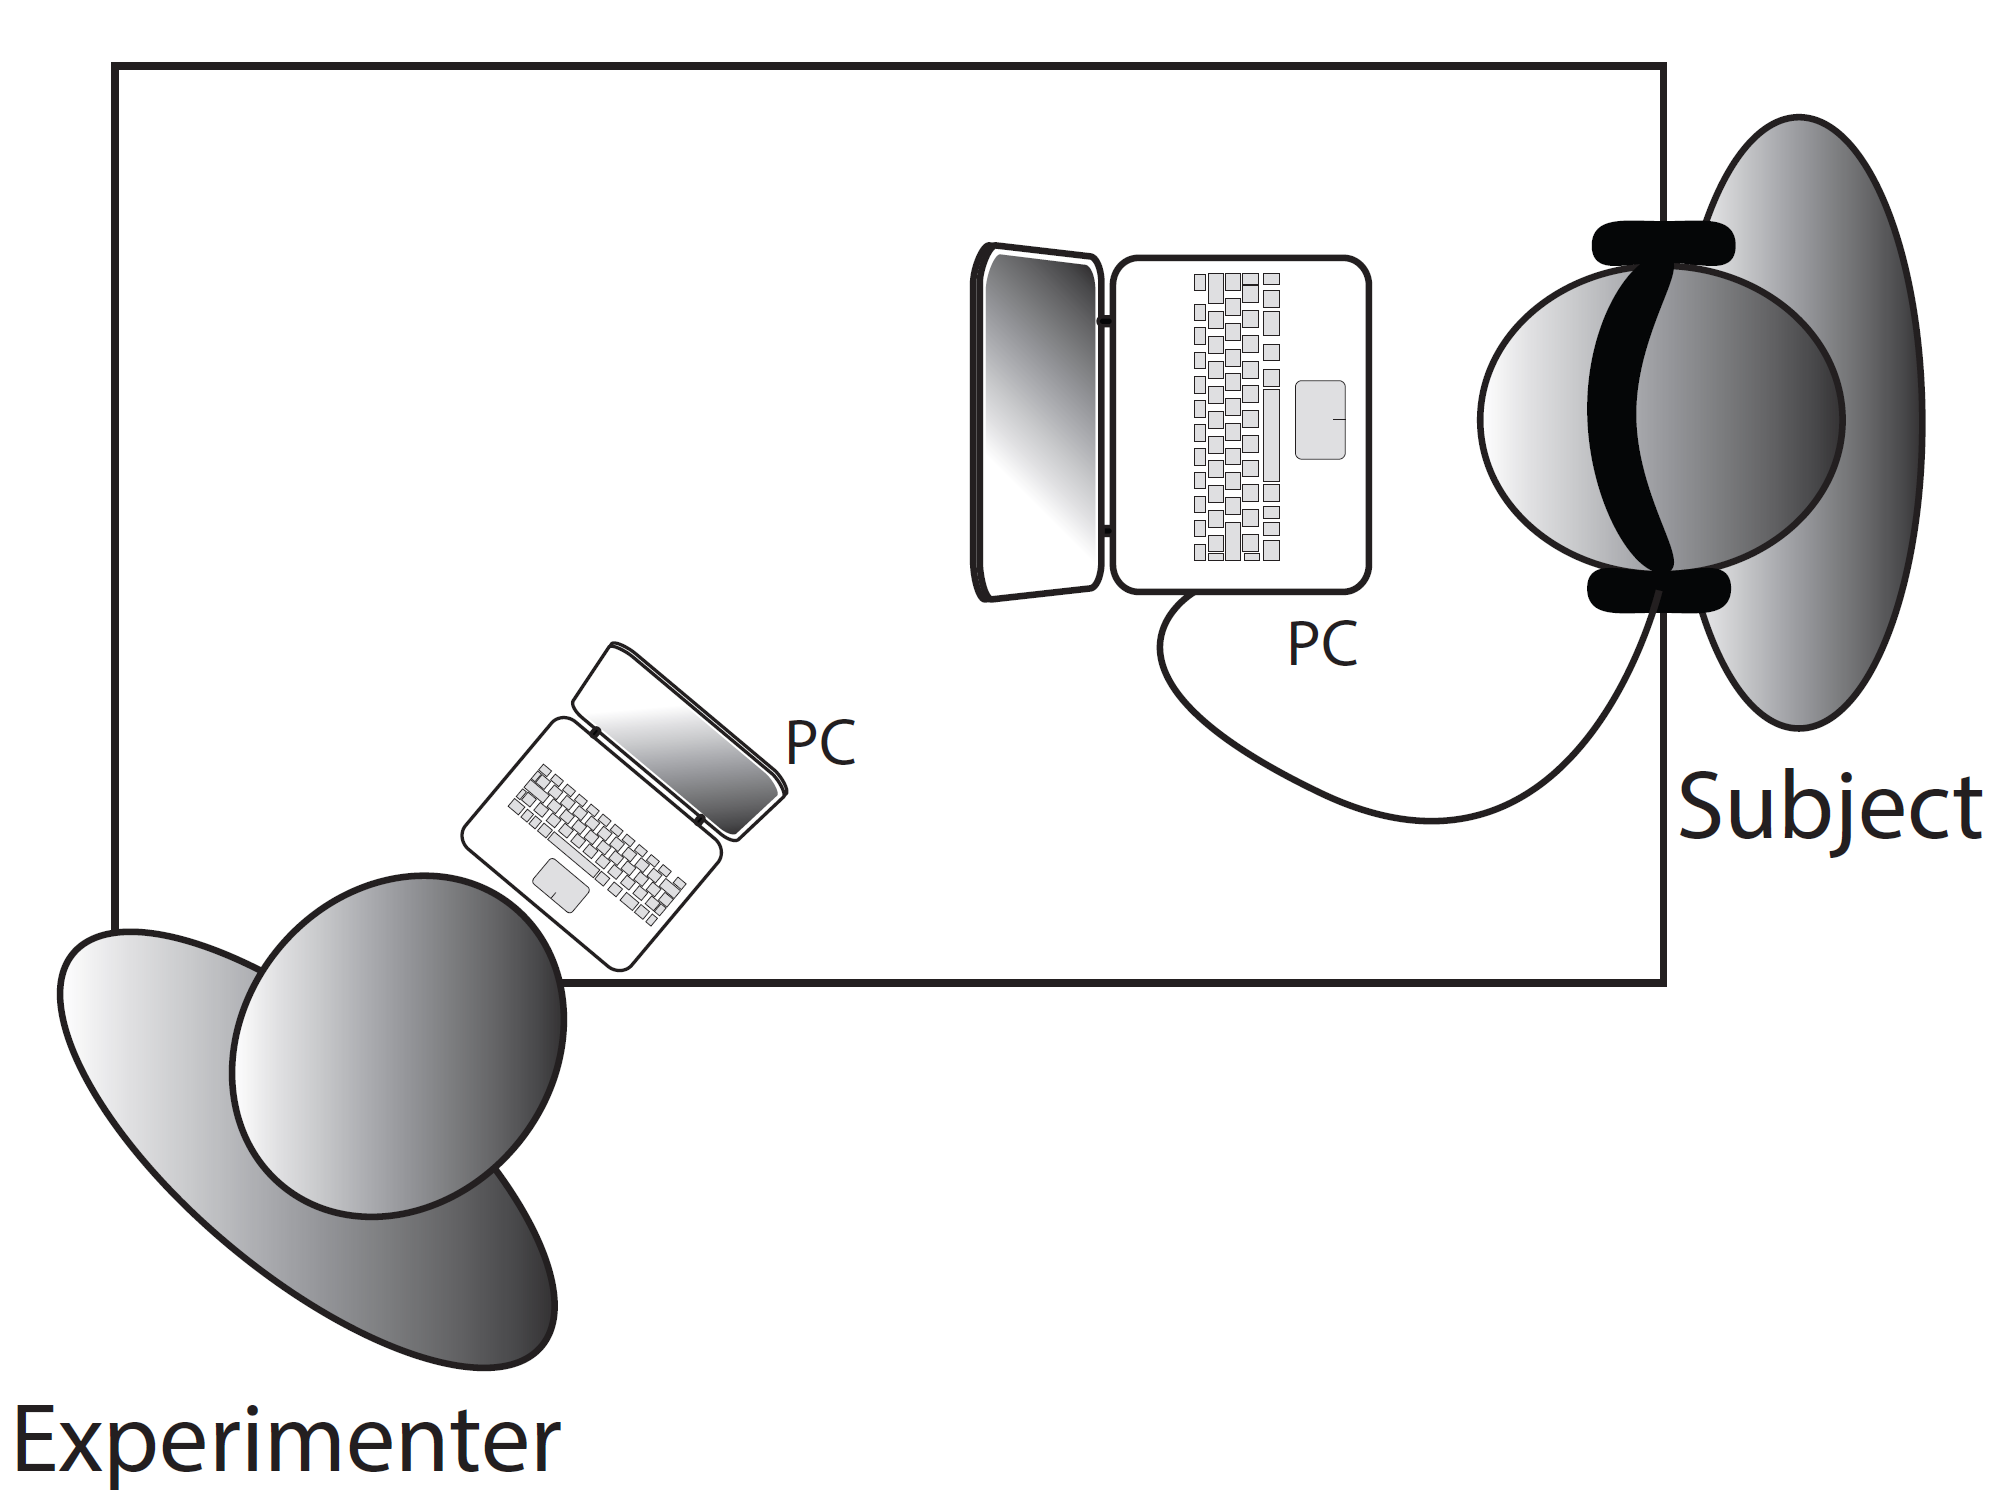
\includegraphics[width = \textwidth]{Figure/Vores_Figurer/experiment.png} 
\caption{A sketch of the experimental setup}
\label{fig:experiment}
\end{figure}

\subsection*{Test subjects}
%
Five test subjects two males and three females, age 23 - 24 (mean: 23.4).

\subsection*{Pilot testing}
%
Based on a pilot test with two test subjects (one male and one female) it is decided to expand the stimuli intensity range down to 0.15 Hz and up to 19.2 Hz.

\section*{Results}
Show data in figures and maybe also tables

OBS: lav funktionerne i hånden eller i excel (de er ikke særlig præcise i MatLab da plot funktionen er lidt forældet.)

\section*{Analysis}
Present the data analysis, show figures, tables and interpret the results.

2-AFC is used and there is a 50 \% chance guessing the right answer of the two possible answers. The point for JND is at 75 \%.

\section*{Discussion and conclusion} 
Compare to other results, discuss the methods used, discuss strange looking data etc. and conclude.
The frequency span used in this study is based on the findings of \citep{Wier1977}. However, there might be other variables affecting the outcomes of this study. These include ambient noise and distractions. Furthermore, they might have used different levels of pitch and more repetitions.

What if a person’s threshold is outside our range of chosen stimuli intensities 

We don’t know if subjects has the same understanding of pitch and how to listen for differences in this. The subjects discussed what they think pitch is, but it is not known if the interpretation of the words used to describe it is understood in the same way.





 
